\chapter{State of the Art}
\label{chap:StateOfTheArt}
\pagestyle{plain}
\vspace{0.5cm}

\noindent This chapter introduces the readers to a complete review of the problem and all the different resolution possibilities.

\section{Physiological signals}
In this section will be defined a general overview on physiological signals that can be used in order to achieve a solution to the Music Emotion Recognition problem.
\\ \indent
Emotions, which affect both human physiological and psychological status, play a very important role in human life. Positive emotions help improve human health and work efficiency, while negative emotions may cause health problems. Long term accumulations of negative emotions are predisposing factors for depression, which might lead to suicide in the worst cases.
\\
The emotion often refers ti a mental state that arises spontaneously rather than through conscious effort and it is accompanied by physical and physiological changes, relevant to the human organs and tissues such as brain, heart, skin, blood flow, muscle, facial expressions, voice, etc. \cite{shu2018review}.
\\ \indent
Emotion recognition has been applied in many areas such as safe driving \cite{de2016enhancing}, health care especially mental health monitoring \cite{guo2013pervasive}, social security \cite{verschuere2006psychopathy}, and so on.
\\
In general, emotion recognition methods could be classified into two major categories:
\begin{itemize}
	\item Using human physical signals such as facial expression \cite{zhang2016facial}, speech \cite{mao2014learning}, gesture, posture, etc. This method has the advantage of easy collecting and is a chapter which has been studied for years. On the other side, the reliability cannot be guaranteed, as it is relatively easy for people to control the physical signals like facial expression or speech to hide real emotions, especially during social communications.
	\item Using internal signals as:
	\begin{itemize}
		\item Electroencephalogram (EEG)
		\item Electrocardiogram (ECG)
		\item Electromyogram (EMG)
		\item Blood Pressure (BP)
		\item Hearth Rate Variability (HRV)
		\item Electrodermal Activity (EDA) as:
		\begin{itemize}
			\item Skin Resistance (SR)
			\item Skin Temperature (ST)
			\item Skin Conductivity (SC)
			\item Galvanic Skin Response (GSR)
		\end{itemize}
		\item Respiration (RSP)
	\end{itemize}
	These signals are produced by the Nervous System which is divided into:
	\begin{itemize}
		\item Central Nervous System (CNS)
		\item Peripheral Nervous System (PNS): consist of the autonomic and somatic nervous systems (ANS and SNS).
	\end{itemize}
	EEG, ECG, EMG, GSR, RSP and GSR change in a certain way when people face some specific situations. Physiological signals are in response to the CNS and ANS. Due to the fact that CNS and ANS are involuntarily activated, they cannot be controlled.
\end{itemize}
In the table \ref{table:biological_signals} is shown a summary of various papers using different biological signals.
\begin{table}[h!]
	\centering
	\begin{tabular}{|l|l|}
		\hline
		Biological signal & Paper\\ [0.5ex] 
		\hline \hline ECG & \cite{dissanayake2019ensemble}, \cite{hsu2017automatic},  \cite{naji2014classification}, \cite{naji2015emotion}, \cite{cai2009research}  \\ 
		\hline ECG, EMG, RSP & \cite{kim2008emotion} \\
		\hline ECG, GSR & \cite{goshvarpour2017accurate} \\ 
		\hline HR, SR & \cite{yoo2005neural} \\
		\hline EEG & \cite{sourina2012real} \\
		\hline HR & \cite{nardelli2015recognizing} \\
		\hline
	\end{tabular}
	\caption{Papers with correspondent biological signal used}
	\label{table:biological_signals}
\end{table}
\newpage
In table \ref{table:physiological_features_relation} is presented the relationship between emotions and physiological features, thanks to \cite{shu2018review}. Arrows indicate increased ($\uparrow$), decreased ($\downarrow$), no change in activation from the baseline ($-$) or both increases and decreases in different studies ($\uparrow\downarrow$).
\begin{table}[h!]
\begin{adjustwidth}{-3cm}{-1cm}
	\centering
	\begin{tabular}{|c|c|c|c|c|c|c|c|}
		\hline
		Signal & Anger & Anxiety & Embarrassment & Fear & Amusement & Happiness & Joy\\ [0.5ex] 
		\hline \hline \textbf{Cardiovascular} &&&&&&& \\ 
		\hline HR & $\uparrow$ & $\uparrow$ &  $\uparrow$ & $\uparrow$ & $\uparrow\downarrow$ & $\uparrow$ & $\uparrow$ \\
		\hline HRV & $\downarrow$ & $\downarrow$ & $\downarrow$ & $\downarrow$ & $\uparrow$ & $\downarrow$ & $\uparrow$ \\
		\hline LF & & $\uparrow$ & & $(-)$ & & $(-)$ & \\
		\hline LF/HF & & $\uparrow$ & & & $(-)$ & & \\
		\hline PWA & & & & $\uparrow$ & & & \\
		\hline PEP & $\downarrow$ & & $\downarrow$ & $\downarrow$ & $\uparrow$ & $\uparrow$ & $\uparrow\downarrow$ \\
		\hline SV & $\uparrow\downarrow$ & $(-)$ & & $\downarrow$ & & $(-)$ & $\downarrow$\\
		\hline CO & $\uparrow\downarrow$ & $\uparrow$ & $(-)$ & $\uparrow$ & $\downarrow$ & $(-)$ & $(-)$ \\
		\hline SBP & $\uparrow$ & $\uparrow$ & $\uparrow$ & $\uparrow$ & $\uparrow$ & $\uparrow$ & $\uparrow$ \\
		\hline DBP & $\uparrow$ & $\uparrow$ & $\uparrow$ & $\uparrow$ & $\uparrow$ & $\uparrow$ & $(-)$\\
		\hline MAP & & & $\uparrow$ & $\uparrow$ & $\uparrow$ & $\uparrow$ & \\
		\hline TPR & $\uparrow$ & & & $\downarrow$ & $\uparrow$ & $\uparrow$ & $(-)$ \\
		\hline FPA & $\downarrow$ & $\downarrow$ & & $\downarrow$ & $\downarrow$ & $\uparrow\downarrow$ & \\
		\hline FPTT  & $\downarrow$ & $\downarrow$ & & $\downarrow$ & & $\uparrow$ & \\
		\hline EPTT & & $\downarrow$ & & $\downarrow$ & & $\uparrow$ & \\
		\hline FT  & $\downarrow$ & $\downarrow$ & & $\downarrow$ & $(-)$ & $\uparrow$ &\\
		\hline \hline \textbf{Electrodermal} &&&&&&& \\ 
		\hline SCR & $\uparrow$ & $\uparrow$ & & $\uparrow$ & $\uparrow$ & & \\
		\hline nSRR & $\uparrow$ & $\uparrow$ & & $\uparrow$ & $\uparrow$ & $\uparrow$ & $\uparrow$ \\
		\hline SCL & $\uparrow$ & $\uparrow$ & $\uparrow$ & $\uparrow$ & $\uparrow$ & $\uparrow$ & $(-)$ \\
		\hline \hline \textbf{Respiratory} &&&&&&& \\ 
		\hline RR & $\uparrow$ & $\uparrow$ & & $\uparrow$ & $\uparrow$ & $\uparrow$ & $\uparrow$ \\
		\hline Ti & $\downarrow$ & $\downarrow$ & & $\downarrow$ & $\downarrow$ & $\downarrow$ & \\
		\hline Te & $\downarrow$ & $\downarrow$ & & $\downarrow$ & & $\downarrow$ & \\
		\hline Pi & $\uparrow$ & & & $\uparrow$ & & $\downarrow$ & \\
		\hline Ti/Ttot & & & & $\uparrow$ & $\downarrow$ & & \\
		\hline Vt & $\uparrow\downarrow$ & $\downarrow$ & & $\uparrow\downarrow$ & $\uparrow\downarrow$ & $\uparrow\downarrow$ & \\
		\hline Vi/Ti & & & & & & $\uparrow$ & \\
		\hline \hline \textbf{Electroencephalography} &&&&&&& \\ 
		\hline PSD($\alpha$ wave) & $\uparrow$ & $\uparrow$ & & $\downarrow$ & $\uparrow$ & $\uparrow$ &  $\uparrow$ \\
		\hline PSD($\beta$ wave) & $\downarrow$ & & & & $\uparrow$ & & \\
		\hline PSD($\gamma$ wave) & & & & $\downarrow$ & $\uparrow$ & $\uparrow$ & $\uparrow$ \\
		\hline DE (avg) & $\uparrow$ & $(-)$ & & $\downarrow$ & & $\uparrow$ & $\uparrow$ \\
		\hline DASM (avg) & $(-)$ & & & $\uparrow$ & $\downarrow$ & $\downarrow$ & $\downarrow$ \\
		\hline RASMs (avg) & $\uparrow$ & & & $\uparrow$ & & $\downarrow$ & \\
		\hline
	\end{tabular}
	\end{adjustwidth}
	\caption{Relationship between emotions and physiological features}
	\label{table:physiological_features_relation}
\end{table}
\newpage
The position of different biosensors is shown in figure \ref{fig:biosensors_position}.
\begin{figure}[h]
    \centering
    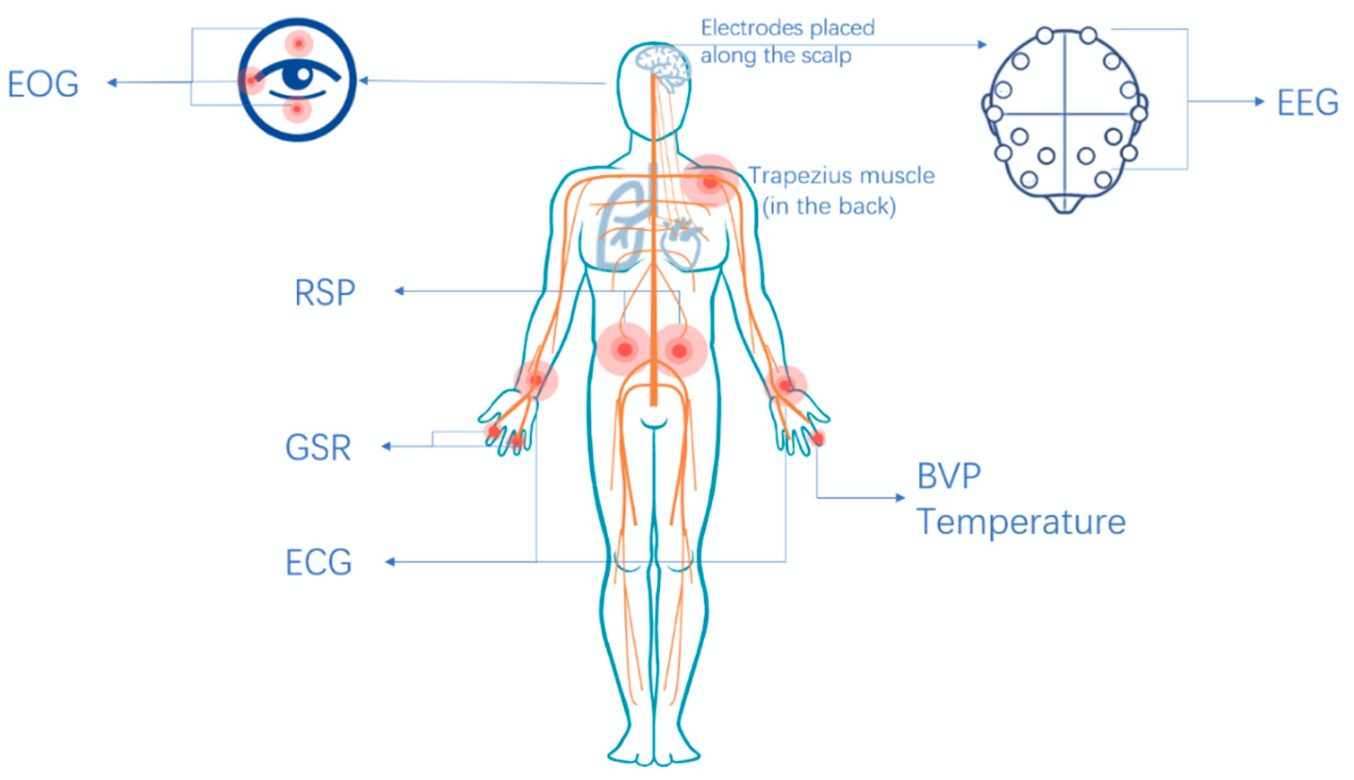
\includegraphics[width=0.8\textwidth]{biosensors_position.png} 
	\caption{Position of the bio-sensors}
    \label{fig:biosensors_position}
\end{figure}

\subsection{Electroencephalogram}
Electroencephalogram (EEG) is an electrophysiological monitoring method to record electrical activity of the brain. EEG measures voltage fluctuations resulting from ionic current within the neurons of the brain. Clinically, EEG refers to the recording of the brain's spontaneous electrical activity over a period of time, as recorded from multiple electrodes placed on the scalp.
\\ \indent
EEG is most often used to diagnose epilepsy, which causes abnormalities in EEG readings.[2] It is also used to diagnose sleep disorders, depth of anesthesia, coma, encephalopathies, and brain death.
\\ 
Many studies have indicated that the physiological correlates of emotions are likely to be found in the central nervous system rather than simply in peripheral physiological responses. Researchers have supported this viewpoint using EEG or other neuroimaging (e.g., functional Magnetic Resonance Imaging) approaches to investigate the specificity of brain activity associated with different emotional states.
\\
However, most of the available studies on emotion-specific EEG response have focused on EEG characteristics at the single-electrode level, rather than at the level of EEG-based functional connectivity.

\subsection{Electrocardiogram}
Electrocardiogram (ECG) is a recording of the electrical activity of the hearth using electrodes placed on the skin. These electrodes detect small electrical changes that are a consequence of cardiac muscle depolarization followed by repolarization during each cardiac cycle, the heartbeat.
\\ \indent
There are three main components to an ECG: the P wave, which represents the depolarization of the atria; the QRS complex, which represents the depolarization of the ventricles; and the T wave, which represents the repolarization of the ventricles, as in figure \ref{fig:ECG}.
\begin{figure}[h]
    \centering
    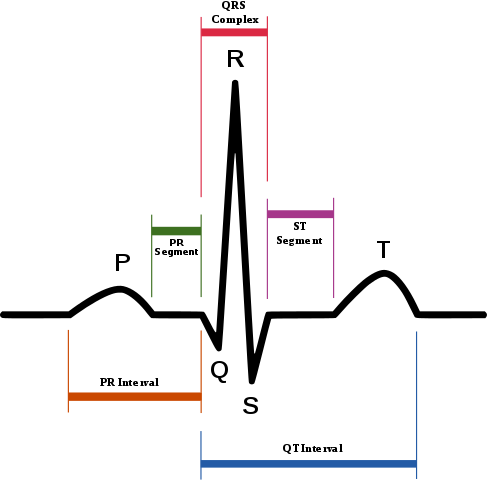
\includegraphics[width=0.6\textwidth]{ECG.png} 
	\caption{ECG of a heart in normal sinus rhythm}
    \label{fig:ECG}
\end{figure}

\subsection{Electromyogram}
Electromyogram (EMG) is an electrodiagnostic medicine technique for evaluating and recording the electrical activity produced by skeletal muscles.
\\
An electromyograph detects the electric potential generated by muscle cells when these cells are electrically or neurologically activated. The signals can be analyzed to detect medical abnormalities, activation level, or recruitment order, or to analyze the biomechanics of human or animal movement.
\\ \indent
Therefore, the best readings are obtained when the sensor is placed on the muscle belly and its positive and negative electrodes are parallel to the muscle fibers. Since the number of muscle fibers that are recruited during any given contraction depends on the force required to perform the movement, the intensity (amplitude) of the resulting electrical signal is proportional to the strength of contraction.
\\ \indent
In psychophysiology, EMG was often used to find the correlation between cognitive emotion and physiological reactions. In the work by Sloan \cite{sloan2004emotion}, for example, the EMG was positioned on the face (jaw) to distinguish \textit{smile} and \textit{frown} by measuring the activity of zygomatic major and corrugator supercilli. In experiment of \cite{kim2008emotion}, bipolar electrodes were placed at the upper trapezius muscle (near the neck) in order to measure the mental stress of the subjects.

\subsection{Hearth Rate Variability}
Hearth Rate Variability (HRV) measure the beat-to-beat temporal changes of the hearth rate, sometimes it is calculated from ECG, but the usability of measuring the ECG is limited. HRV can be evaluatd also through the Blood Volume Pulse (BVP) or Photoplethysmography (PPG).
\\ \indent
A reduced HRV is linked to psychiatric illness as depression, anxiety. The heart rate is the most natural choice for arousal detection using comparison of sympathetic and parasympathetic frequency bands of the time series. However, it is highly dependent on the position of the body during monitoring.

\subsection{Electrodermal Activity}
As already been studied in chapter \ref{chap:TheoreticalBackgroundEDA}, EDA measures the resistance of the skin and the skin conductivity applying electrodes to the skin. The skin conductivity decreases during relaxed states, and increase when exposed to effort.

\subsection{Respiration}
Respiration (RSP) is the process of moving air into an out of the lungs to facilitate gas exchange with the internal environment, mostly bringing in oxygen and flushing out carbon dioxide.
\\
The respiration can be measured with a latex rubber band, the amount of stretch in the elastic is measured as a voltage change and recorded. The most common measures of RSP are the depth of breathing and the rate of RSP.
\\ \indent
RSP rate generally decreases with relaxation, tense situations may result in momentary RSP cessation. Irregularity in the RSP pattern could be the cause of negative emotions.
\\
Due to the fact that RSP is closely linked to the cardiac function, RSP can be affect other measures like EMG and SC measurements.
\\
Positions to the left, and typical waveform of the signals to the right are presented in the figure \ref{fig:waveform_biosensors}.
\begin{figure}[h]
    \centering
    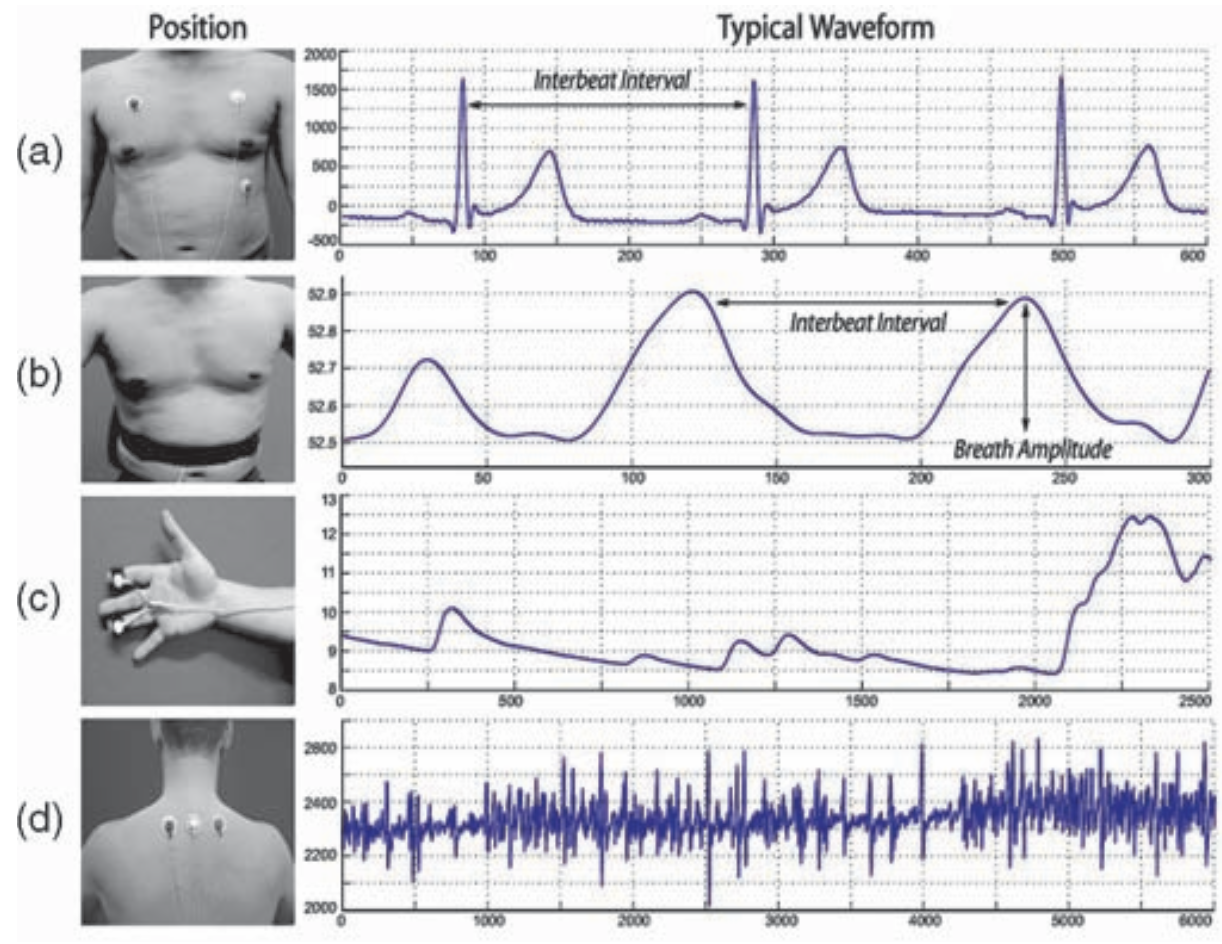
\includegraphics[width=0.8\textwidth]{waveform_biosensors.png} 
	\caption{Positions (left) and waveform of the signals (right), (a) ECG, (b) RSP, (c) SC, (d) EMG}
    \label{fig:waveform_biosensors}
\end{figure}

\section{General methodology}
For physiological signal-based emotion recognition, there is a common methodology which can be divided into two categories:
\begin{itemize}
	\item Traditional Machine Learning methods: model specific methods, which require carefully designed hand-crafted features and feature optimization methods.
	\item Deep learning methods, model-free methods, which can learn the inherent principle of the data and extract features automatically.
\end{itemize}
The whole emotion recognition framework is shown in figure \ref{fig:emotion_recognition_process}.
\begin{figure}[h]
    \centering
    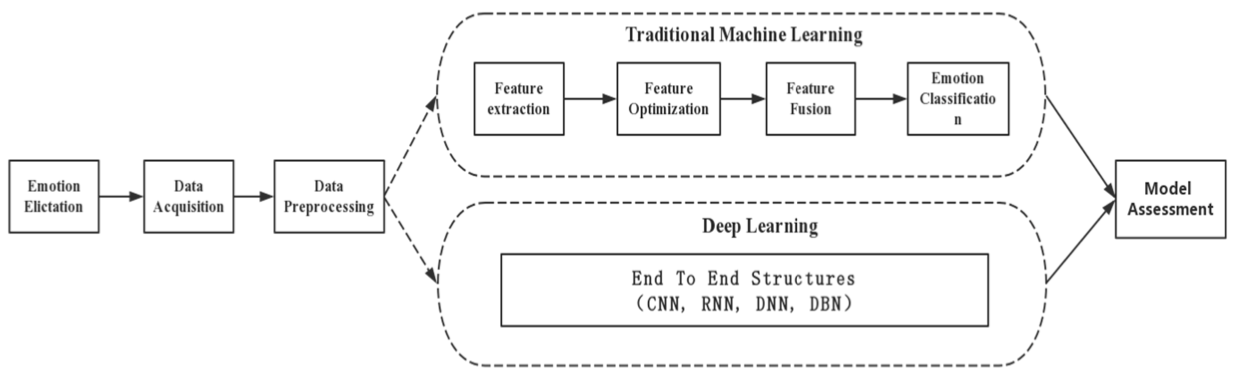
\includegraphics[width=\textwidth]{emotion_recognition_process.png} 
	\caption{Emotion recognition process using physiological signals under targer emotion stimulation}
    \label{fig:emotion_recognition_process}
\end{figure}

\subsection{Preprocessing}
After the part of data acquisition, which is different for each physiological signal, there is the data preprocessing step. It is necessary to eliminate the noise effect, artifacts and other signal parts that may lead to wrong results. Due to the complex and subjective nature of raw physiological signals and the sensitivity to noises, electromagnetic interferences, movement artifacts, ... this step is mandatory.
\\ \indent
Some of the common steps can be summarized in:
\begin{itemize}
	\item Filtering: is commonly used a low-pass filter to remove noises, or also adaptive bandpass filters to remove artifacts.
	\item Discrete Wavelet Transform (DWT): used to reduce the noise of physiological signals
	\item Independent Component Analysis (ICA): used to extract and remove respiration sinus arrhythmia from ECG.
	\item Empirical Mode Decomposition (EMD): used to remove the eye-blink from EEG.
\end{itemize}

\subsection{Traditional Machine Learning}
Main steps for traditional ML methods, as already presented in \ref{ML}. There are processes including feature extraction, feature selection and classification.

\paragraph{Feature extraction}
\mbox{} \\ \\ \indent
Feature extraction plays a fundamental role in the emotion recognition model. Several major features are extracted for each physiological signal, because is important to extract the most prominent features for emotion recognition. For example EEG is a complex and non-stationary signal, so some statistical features like Power Spectral Density (PSD) and Spectral Entropy (SE) are commonly used.
\\
Often are extracted statistical features as mean, standard deviation, Kurtosis, Skewness, entropy.
\\
However, each bio-signal has to be investigated separately as extracted features might vary in their usefulness for the classification of emotions.

\paragraph{Feature selection}
\mbox{} \\ \\ \indent
After the feature extraction process, there might be a quantity of features, some of which may be irrelevant, some that are probably correlated each other, there might be some redundant features.
\\
It lead to a long time of analyzing the features and train the model and it is easy to produce overfitting problem and another problem of sparse features, called \textit{curse of dimensionality}, which results in the decrease of the model performance.
\\
Some of the main feature selection algorithms are RfeliefF, MRmR, Sequential Backward Selection (SBS) and Sequential Forward Selection (SFS), PCA, ...
\\ \indent
In general there are several feature selection alforithms, some reduce the dimensionality by taking out some redundant or irrelevant featuresm other transform the original one into a new set of features. Performances of the feature selection algorithm depends on the classifier and the dataset, due to this, the perfect feature selection algorithm do not exist.

\paragraph{Classification}
\mbox{} \\ \\ \indent
In emotion recognition, the major task is to assign the input signal to one of the given class sets. There are several classification models like Linear Discriminant Analysis (LDA), k-Nearest Neighbor (kNN), Support Vector Machine (SVM), Random Forest (RF), ...

\subsection{Deep Learning}
Deep Learning (DL) methods have the benefits to be model-free methods, so they do not depends on the specific model considered.
\\
Examples of DL algorithms are Convolutional Neural Network (CNN), Recurrent Neural Network (RNN), ... Neural network in general are particular types of ML methods which have as fundamental unit the node, loosely based on the biological neuron. 
\\ \indent
The relevant aspect of DL is that it can learn the inherent principle of the data and extract features automatically, so there is no need to extract feature and select the most relevant ones, which could lead to a better generalization of the problem.

\subsection{Model assessment and selection}
The generalization error of the classifier can be evaluated by experiments, where a testing set should be used to test the ability of the classifier to classify the new samples, and the testing error on the testing set could be viewed approximately as the generalization error.
\\
The dataset is divided into two mutually exclusive sets, the training and the testing set. It is important to maintain the consistency of the data distribution as much as possible. In general, the experiment need to repeat several times with random division and then calculate the average value as the evaluation result.
\\ \indent
There is also k-fold crossing-validation. the initial sampling is divided into $K$ sub-samples. One sub-sample is used as the testing set and the other $K-1$ samples are used for training. Cross-validation is repeated K-times. Each sub-sample is validate once and the average result of K times is used as the final result. The most common is the 10-fold cross-validation.
\\ \indent
To evaluate the performance of the experiment there is the accuracy, which is the proportion of samples that are correctly classified to the total samples.

\section{Issues of physiological signals}
A lot of efforts have been made in revealing the relationships between explicit physiological signals and implicit psychological feelings. However, there are still several challenges in emotion recognition based on physiological signals:
\begin{itemize}
	\item Need a very well designed setup in order to obtain high quality physiological data. The standard setup is the standard lab setting with subjects with earphones  sit motionless in front of a screen where the emotion stimuli materials are played. This system is fixed, data are noiseless and stable, but the issue of obtaining genuine emotions which is dependent heavily on the emotion stimulated materials is hard to deal with it.
	\item The stimulus materials are artificially selected, labels of the materials are manually set, while for the same thing human emotions vary from each other, this may lead to a large deviation in the rating of the material. In \cite{muhl2011modality}, the author showed that different introduction ways led to different physiological responses.
	\item There is no still clear evidence that what feature combination of what physiological signal combinations are the most significantly relevant to emotion changes.
	\item For most studies, the number of subjects is small. Due to limited samples, the performance of the classifier with subjects who have not been trained would be poor. The clear efficient method is to include more subjects from different ages and backgrounds.
	\item Emotion perception and experience lead to strong differences.
	\item The reliability of facial expressions cannot be guaranteed sometimes.
\end{itemize}

\section{Related works}
In this section will be presented some works done during the last years on all physiological signals that tries to understand the relationship of physiology and human emotions.

\subsection{ECG and GSR signal emotion recognition}
In the work \cite{goshvarpour2017accurate} Electrocardiogram and Galvanic Skin Response of 11 healthy students were collecred while subjects were listening to emotional music clips. They extracted Matching Pursuit (MP) coefficients frin ECG and GSR signals.
\\ \indent
Than were calculated some statistical indices from the MP coefficients and three dimensionality reduction method were applied, PCA, LDA and Kernel PCA. These features were fed into the Probabilistic Neural Network (PNN) in subject-dependent and subject-independent modes.
\\ \indent
The PNN is feed with a feature vector in the input layer, is determined a distance between the input and the weight vector. Is calculated the summation of these contributions for each input class to yield the probability. Finally is selected the maximum of these probabilities by a competitive layer and assigned $1$ for that class and $0$ elsewhere.
\\ \indent
They achieved, using PCA, the highest recognition rate of 100\% for $\sigma = 0.01$.

\subsection{ECG sensors for human emotion recognition}
The research of \cite{dissanayake2019ensemble}, they suggest an ensamble learning approach for developing a machine learning model that can recognize four major human emotions (anger, sadness, joy and pleasure) incorporating ECG signals.
\\ \indent
As feature extraction method, the analysis combines four ECG signals techniques. Several ML methods have been applied to the model, the most accurate (with an accuracy of 70\% is achieved by using an Extra Tree Classifier (a variant of the Random Forest that introduce more variation in the ensemble).

\subsection{Automatic ECG emotion recognition}
In \cite{hsu2017automatic} is presented an automatic ECG-based emotion recognition algorithm. They recorded ECG signal from subjects and extracted some features from the signal from the time and frequency domain. Than performed an algoritm of feature selection, a sequential forward floating selection-kernel-based class separability-based.
\\
Valence and arousal and four types of of emotions are recognized using Least Square-Support Vector Machine recognizer. They gained a classification rate for positive/negative valence, high/low arousal, and four types of emotion classification tasks are 82.78\%, 72.91\%, and 61.52\%, respectively.

\subsection{Classification of music emotions with  forehead biosignals and ECG}
In the work of \cite{naji2014classification} to recognize music-induced emotions is used a fusion of three-channel forehead biosignals (left and right temporal channel and frontalis) and ECG. They employed two parallel SVM as arousal and valence classifiers.
\\ \indent
The inputs of the classifiers were obtained by applying a fuzzy-rough model feature evaluation criterion and sequential forward floating selection algorithm.
\\
The average classification accuracy was of 88.78\% (valence classification accuracy of 94.91\% and arousal classification accuracy of 93.63\%).

\subsection{Emotion classification with forehead biosignals}
In \cite{naji2015emotion} investigates the feasibility of usign 3-channel forehead bisignals. Classification in vale-arousal space is performed by employing two parallel cascade-forward Neural Networks.
\\
The inputs of the classifiers were obtained by applying a fuzzy rough model feature evaluation criterion and sequential forward floating selection algorithm. An averaged classification accuracy of 87.05\% was achieved, corresponding to average valence classification accuracy of 93.66 \% and average arousal classification accuracy of 93.29 \%.






